\chapter{Arhitektura i dizajn sustava}

		\textit{Arhitektura je podjeljena na tri sustava:}
	\begin{itemize}
		\item 	\textit{Web Aplikacija}
		\item 	\textit{Web Poslužitelj}
		\item 	\textit{Baze podataka}		
	\end{itemize}
	
	%unos slike
			\begin{figure}[H]
				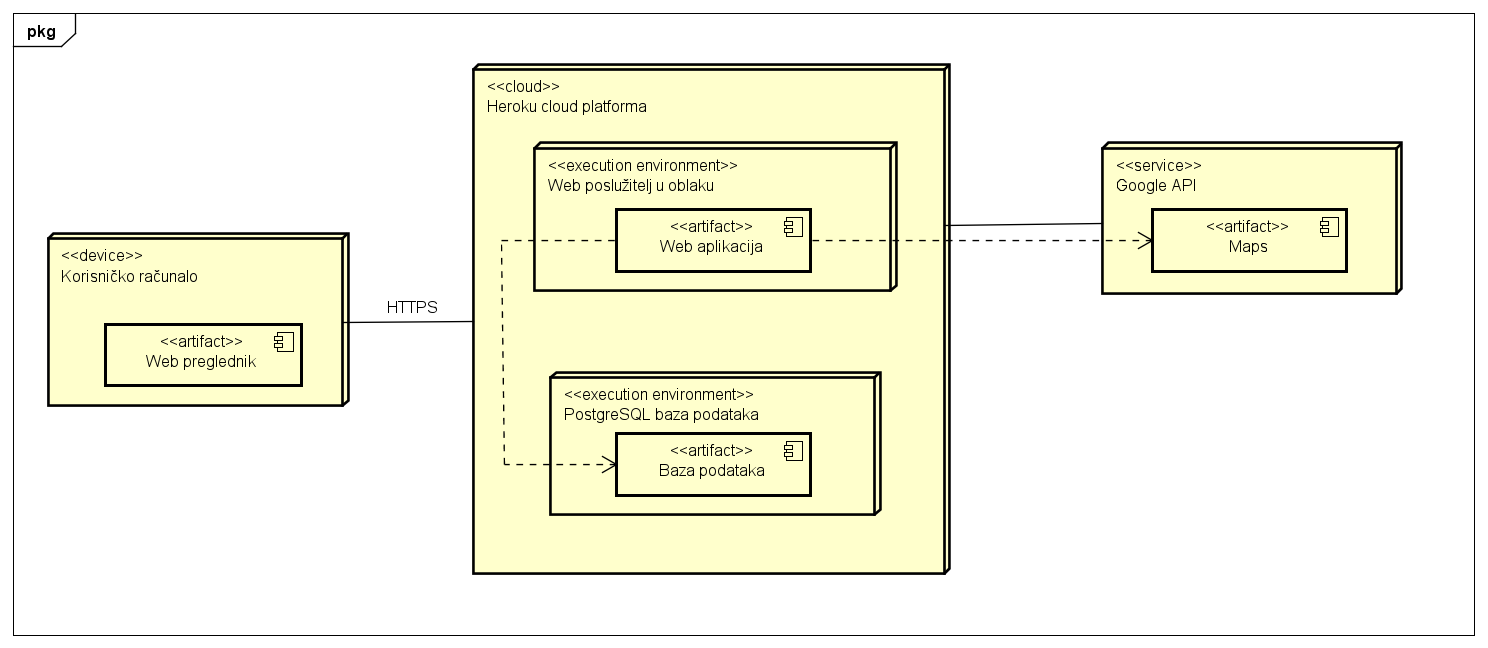
\includegraphics[scale=0.4]{dijagrami/dijagram_razmjestaja.png} %veličina slike u odnosu na originalnu datoteku i pozicija slike
				\centering
				\caption{Dijagram arhitekture sustava}
				\label{fig:promjene}
			\end{figure}

		Korisnik aplikaciji pristupa preko web preglednika. \textit{Web preglednik} je program kojim korisnik pristupa web sadržaju. Jedna od njegovih glavnih zadaća je prevođenje koda u konačni produkt sa svim sadržajima namijenjen korisniku. 
		
		Pošto je aplikacija dinamička, preglednik komunicira s web aplikacijom preko \textit{web poslužitelja}, odnosno servera, čija je glavna zadaća prosljeđivanje korisničkih zahtjeva aplikaciji. Ta komunikacija odvija se preko HTTPS protokola kako bi se omogućio siguran prijenos korisnikovih podataka i informacija.
		
		\textit{Web aplikacija} obrađuje te zahtjeve, pristupa bazi podatka i ostalim vanjskim servisima po potrebi te šalje odgovor na korisinkov zahtjev u obliku HTML dokumenta razmuljiv web pregledniku. Ako se zahtjev nije uspio izvršiti, aplikacija će korinsiku dojaviti pogrešku. 
		
		\textit{Baza podataka} služi za pohranu, izmjenu i dohvat podataka koji će se obrađivati u aplikaciji. Za njenu implementaciju koristiti ćemo Postgresql.
	
		Za izradu web aplikacije odlučili smo koristiti Node.js, te ćemo većinu funkcionalnosti aplikacije ostvariti uz pomoć Express frameworka te Pug HTML template enginea. Za spajanje aplikacije s bazom podataka koristiti ćemo Connect-pg-Simple.
		
			Aplikaciju ćemo razvijati
		u razvojnom okruženju Microsoft Visual Studio. 
			Arhitektura sustava temeljit će se na 
		Model-View-Controller (MVC) arhitekturi. 
		
		
		\newpage
				
		\section{Baza podataka}
			
			Za naš sustav koristiti ćemo relacijsku bazu podataka, ostvarenu u aplikaciji Postgresql. Baza je prilagođena brzom pohranjivanju i dohvaćanju podataka, te su entiteti napravljeni tako da odgovaraju modelima u dijagramu razreda.
			
				Baza podataka sastoji se od sljedećih entiteta:
				\begin{itemize}
					\item 	\textit{Korisnik}
					\item 	\textit{Tvrtka}
					\item 	\textit{Parking}
					\item 	\textit{Vozilo}
					%		\item 	\textit{Vozi}
					\item 	\textit{Rezervacija}
					\item 	\textit{Sjednica}
				\end{itemize}
		
			\subsection{Opis tablica}
			

				
				\textbf{Korisnik}  je entitet koji čuva informacije o korisniku aplikacije \textit{ParkirajMe}. Sadrži atribute: Korisničko ime i OIB korisnika, broj kreditne kartice, e-mail korisnika, te njegovo ime i prezime. Ovaj entitet u vezi je \textit{One-to-Many} s entitetom vozilo preko korisničkog imena, zato jer svaki korisnik može posjedovati više vozila, a jedno vozilo također može imati više korisnika koji ga parkiraju.
				


				\begin{longtabu} to \textwidth {|X[10, l]|X[6, l]|X[20, l]|}
					
					\hline \multicolumn{3}{|c|}{\textbf{korisnik}}	 \\[3pt] \hline
					\endfirsthead
					
					\hline \multicolumn{3}{|c|}{\textbf{korisnik}}	 \\[3pt] \hline
					\endhead
					
					\hline 
					\endlastfoot
					

					Korisničko ime	& VARCHAR &		Jedinstveno korisničko ime korisnika   	\\ \hline 
					Lozinka	& VARCHAR &		Hash jedinstvene lozinke korisnika   	\\ \hline 
					OIB & CHAR(11)	&  	Osobni identifikacijski broj korisnika 	\\ \hline
					Broj kred. kartice	& VARCHAR &   	Broj kreditne kartice korisnika	\\ \hline 
					Email & VARCHAR & 		adresa elektroničke pošte korisnika  \\ \hline 
					Ime & VARCHAR	&  		Ime korisnika	\\ \hline 
					Prezime	& VARCHAR &		Prezime korisnika   	\\ \hline 
					Razina ovlasti	& INT &		Razina ovlasti korisnika   	\\ \hline 
					
					
				\end{longtabu}
			
			\textbf{Tvrtka} je entitet koji predstavlja korisnički račun tvrtke koji je u njeno ime otvorio ovlašteni zaposlenik tvrtke. Sadrži atribute: korisničko ime, lozinka, OIB tvrtke, Email , ime te adresu sjedišta. Povezan je vezom \textit{One-To-Many} s entitetom parking, zato jer je jedna tvrtka može imati više parkinga.
			
			
				\begin{longtabu} to \textwidth {|X[10, l]|X[6, l]|X[20, l]|}
				
				\hline \multicolumn{3}{|c|}{\textbf{tvrtka}}	 \\[3pt] \hline
				\endfirsthead
				
				\hline \multicolumn{3}{|c|}{\textbf{tvrtka}}	 \\[3pt] \hline
				\endhead
				
				\hline 
				\endlastfoot
				
				\cellcolor{green}Korisničko ime	& VARCHAR &		Jedinstveno korisničko ime ovlaštenog zaposlenika tvrtke   	\\ \hline 
				Lozinka	& VARCHAR &		Hash jedinstvene lozinke ovlaštenog zaposlenika tvrtke   	\\ \hline 
				OIB tvrtke & CHAR(11)	&  	Osobni identifikacijski broj tvrtke 	\\ \hline
				Email & VARCHAR & 		adresa elektroničke pošte tvrtke  \\ \hline 
				Ime & VARCHAR	&  		Ime tvrtke	\\ \hline 
				\cellcolor{LightBlue} adresaTvrtka	& VARCHAR &		Adresa sjedišta tvrtke   	\\ \hline 
				
				
			\end{longtabu}
		
		\textbf{Vozilo} je entitet koji pohranjuje koja sve vozila je u aplikaciju unio neki korisnik, te su to jedina dva atributa ovog entiteta. U vezi je \textit{Many-to-One} s entitetom korisnik preko atributa korisničko ime, te u vezi \textit{One-to-Many}  s entitetom rezervacija preko atributa registracija.
		
			\begin{longtabu} to \textwidth {|X[10, l]|X[6, l]|X[20, l]|}
				
				\hline \multicolumn{3}{|c|}{\textbf{vozilo}}	 \\[3pt] \hline
				\endfirsthead
				
				\hline \multicolumn{3}{|c|}{\textbf{ozilo}}	 \\[3pt] \hline
				\endhead
				
				\hline 
				\endlastfoot
				
				Korisničko ime	& VARCHAR &		Jedinstveno korisničko ime vlasnika vozila   	\\ \hline 
				Registracija	& VARCHAR &		Registracija automobila   	\\ \hline 
			 
				
				
				
			\end{longtabu}
		
		\textbf{Rezervacija} je entitet koji sadržava podatke o rezervaciji jednog parkirnog mjesta. Njezini atributi su: ID rezervacije, ID grupe rezervacija kojoj ova rezervacija pripada,  Korisničko ime onog tko je rezervirao, registracija vozila, ID parkinga, datum i vrijeme početka i kraja rezervacije. Povezan je vezom \textit{Many-to-One} sa entitetom Vozilo preko atributa Korisničko ime i rezervacija (Ključ entiteta vozilo), te s entitetom Parking vezom \textit{Many-to-One} preko atributa Parking ID.
			
			\begin{longtabu} to \textwidth {|X[10, l]|X[6, l]|X[20, l]|}
				
				\hline \multicolumn{3}{|c|}{\textbf{rezervacija}}	 \\[3pt] \hline
				\endfirsthead
				
			%	\hline \multicolumn{3}{|c|}{\textbf{rezervacija}}	 \\[3pt] \hline
			%	\endhead
				
			%	\hline 
				\endlastfoot
				
				\cellcolor{green}IDRezervacija	& SERIAL &		Jedinstveni ID rezervacije  	\\ \hline 
				ID grupe	& INT &		Jedinstvena oznaka grupe rezervacija  	\\ \hline
				Korisničko ime	& VARCHAR &		Jedinstveno korisničko ime vlasnika vozila   	\\ \hline
				Registracija vozila	& VARCHAR &		Registracija automobila koji će zauzeti mjesto   	\\ \hline 
				IDParking	& INT &		Jedinstvena oznaka parkinga  	\\ \hline 
				Pocetak rezervacije & TIMESTAMP	&  	Početak rezervacije 	\\ \hline
				Kraj rezervacije & TIMESTAMP & 		Završetak rezervacije  \\ \hline 
				
				
				
			\end{longtabu}
		
		\textbf{Parking} je entitet koji sadržava podatke o jednom parkingu. Njegovi atributi su: ID parkinga, OIB tvrtke koja ga je objavila, ukupan kapacitet, broj slobodnih mjesta, cijena parkirnog mjesta, adresa parkinga, te geografska širina i dužina njegove lokacije. Povezan je sa entitetom tvrtka vezom \textit{Many-to-One} pošto jedna tvrtka može imati više parkinga, te s entitetom rezervacije vezom \textit{One-to-Many} zato jer na jednom parkingu može biti više rezervacija. Također je povezan s entitetom Lokacija vezom \textit{One-to-One} preko atributa ID lokacija.
		
		\begin{longtabu} to \textwidth {|X[10, l]|X[6, l]|X[20, l]|}
			
			\hline \multicolumn{3}{|c|}{\textbf{parking}}	 \\[3pt] \hline
			\endfirsthead
			
			\hline \multicolumn{3}{|c|}{\textbf{parking}}	 \\[3pt] \hline
			\endhead
			
			\hline 
			\endlastfoot
			
			
			ID parkinga	& SERIAL &		Jedinstvena oznaka parkinga   	\\ \hline
			Korisničko ime tvrtke	& VARCHAR & korisničko	ime tvrtke koja je vlasnik parkinga  	\\ \hline 
			Kapacitet	& INT &		Ukupan kapacitet parkinga 	\\ \hline 
			Broj slob. mjesta & INT	&  	Broj slobodnih mjesta na parkingu 	\\ \hline
			Cijena po satu & NUMERIC & 		Cijena rezervacije parkinga po satu  \\ \hline 
			ID lokacija	& INT & Jedinstvena oznaka lokacije parkinga 	\\ \hline
			
		\end{longtabu}
	
		
		
			\textbf{Lokacija} je entitet koji sadržava podatke o jednoj lokaciji. Njegovi atributi su ID lokacije, njena adresa,  te geografska širina i dužina. Povezan je vezom \textit{One-to-One} s entitetom Parking zato jer se na jednoj lokaciji može nalaziti samo jedan parking.
			
			\begin{longtabu} to \textwidth {|X[10, l]|X[6, l]|X[20, l]|}
			
				\hline \multicolumn{3}{|c|}{\textbf{lokacija}}	 \\[3pt] \hline
				\endfirsthead
				
				\hline \multicolumn{3}{|c|}{\textbf{lokacija}}	 \\[3pt] \hline
				\endhead
				
				\hline 
				\endlastfoot
				
				
				ID lokacije	& SERIAL &		Jedinstvena oznaka lokacije  	\\ \hline
				Adresa lokacije	& VARCHAR & Adresa lokacije 	\\ \hline 
				Geo. širina & NUMERIC	&  	Geograska širina lokacije 	\\ \hline
				Geo. dužina & NUMERIC	&  	Geograska dužina lokacije 	\\ \hline
				
	
		\end{longtabu}
	
		\textbf{Sjednica} je entitet koji sadrži informacije o sjednicama koje se stvaraju na stranici ParkirajMe. Sadrži atribute ID sjednice, informacije o sjednici ti vrijeme trajanja sjednice.
		
		\begin{longtabu} to \textwidth {|X[10, l]|X[6, l]|X[20, l]|}
			
			\hline \multicolumn{3}{|c|}{\textbf{sjednica}}	 \\[3pt] \hline
			\endfirsthead
			
			\hline \multicolumn{3}{|c|}{\textbf{sjednica}}	 \\[3pt] \hline
			\endhead
			
			\hline 
			\endlastfoot
			
			
			ID sjednice	& VARCAHR &		Jedinstvena oznaka sjednice  	\\ \hline
			Info	& JSON & Informacije o sjednici	\\ \hline 
			Trajanje & TIMESTAMP	&  	Trajanje sjednice	\\ \hline

			
			
		\end{longtabu}
	
			\subsection{Dijagram baze podataka}
										
					%unos slike
				\begin{figure}[H]
					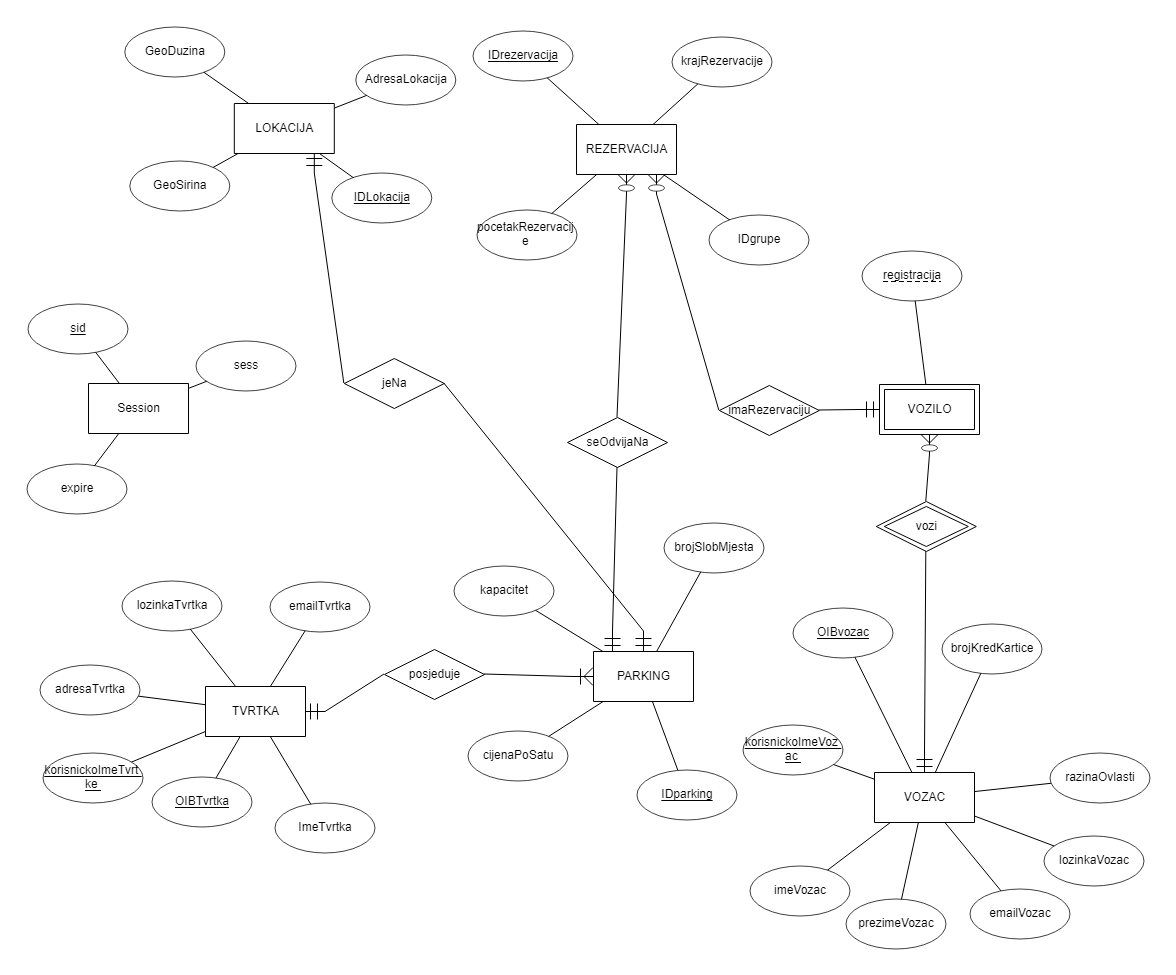
\includegraphics[scale=0.4]{dijagrami/ParkirajMeERModel.png} %veličina slike u odnosu na originalnu datoteku i pozicija slike
					\centering
					\caption{ER model}
					\label{fig:promjene}
				\end{figure}
				

				%unos slike
				\begin{figure}[H]
					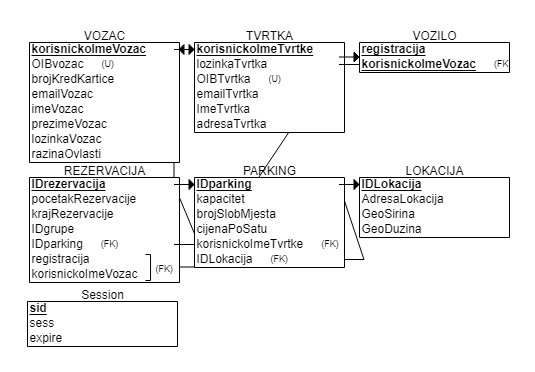
\includegraphics[scale=0.8]{dijagrami/ParkirajMeRelShema.png} %veličina slike u odnosu na originalnu datoteku i pozicija slike
					\centering
					\caption{relacijska shema}
					\label{fig:promjene}
				\end{figure}


			

			\eject
			
			
		\section{Dijagram razreda}
		
			Dijagrami razreda MVC arhitketure sustava prikazani su na slikama 4.4, 4.5 i 4.6.\\
			Razredi na slici 4.3 predstavljaju klase modela, koji su uglavnom direktno povezani s entitetima u bazi podataka. \\
			Razredi na slici 4.4 su pomoćne klase koje pomažu upravljanju podatcima, te najčešće služe za komunikaciju s bazom podataka.\\
 		    Na slici 4.5 se vide razredi koji implementiraju funkcionalnosti \textit{routera}\footnote{https://expressjs.com/en/guide/routing.html}. Oni prikazuju pug\footnote{https://pugjs.org/api/getting-started.html} datoteke koje određuju sadržaj i izgled web stranice.
			\newline
			Razred \textbf{Korisnik} predstavlja bilo kojeg korisnika aplikacije, bio to vozač, tvrtka, administrator ili ne-registrirani korisnik. \textbf{Vozač} predstavlja korisnika aplikacije koji želi rezervirati parirališno mjesto, a \textbf{Tvrtka} korisnika koji želi iznajmljivati svoju parkirališnu površinu. \textbf{Administrator} je korisnik s najvećim ovlastima na aplikaciji. 
			Klasa \textbf{Rezervacija} u sebi pohranjuje informacije o registracijama, kojih postoji 3 različite vrste (jednokratne, ponavljajuće i trajne) koje se označuju atributom \textbf{idgrupe} koja označava pripadajuću vrstu rezervacije:
			\begin{itemize}
				\item jednokratna 	= 0
				\item ponavljajuća 	= 1
				\item trajna 		= 2
			\end{itemize}
			
			%unos slike
			\begin{figure}[H]
				\includegraphics[scale=0.4]{dijagrami/modeli.png} %veličina slike u odnosu na originalnu datoteku i pozicija slike
				\centering
				\caption{Dijagram razreda za modele}
				\label{fig:promjene}
			\end{figure}
		
		
			Pomoćne klase su klase koje u sebi sadrže pomoćne funkcije koje potpomažu ostvarivati funkcionalnosti drugih klasa, te većina služi za direktno slanje upita bazi podataka. Klasa \textbf{datePicker} služi za prikaz izbornika datuma, dok \textbf{displayLocations} služi za prikaz karte preko \textit{Google Maps APIa}, te prikaz lokacija na karti.
			
			%unos slike
			\begin{figure}[H]
				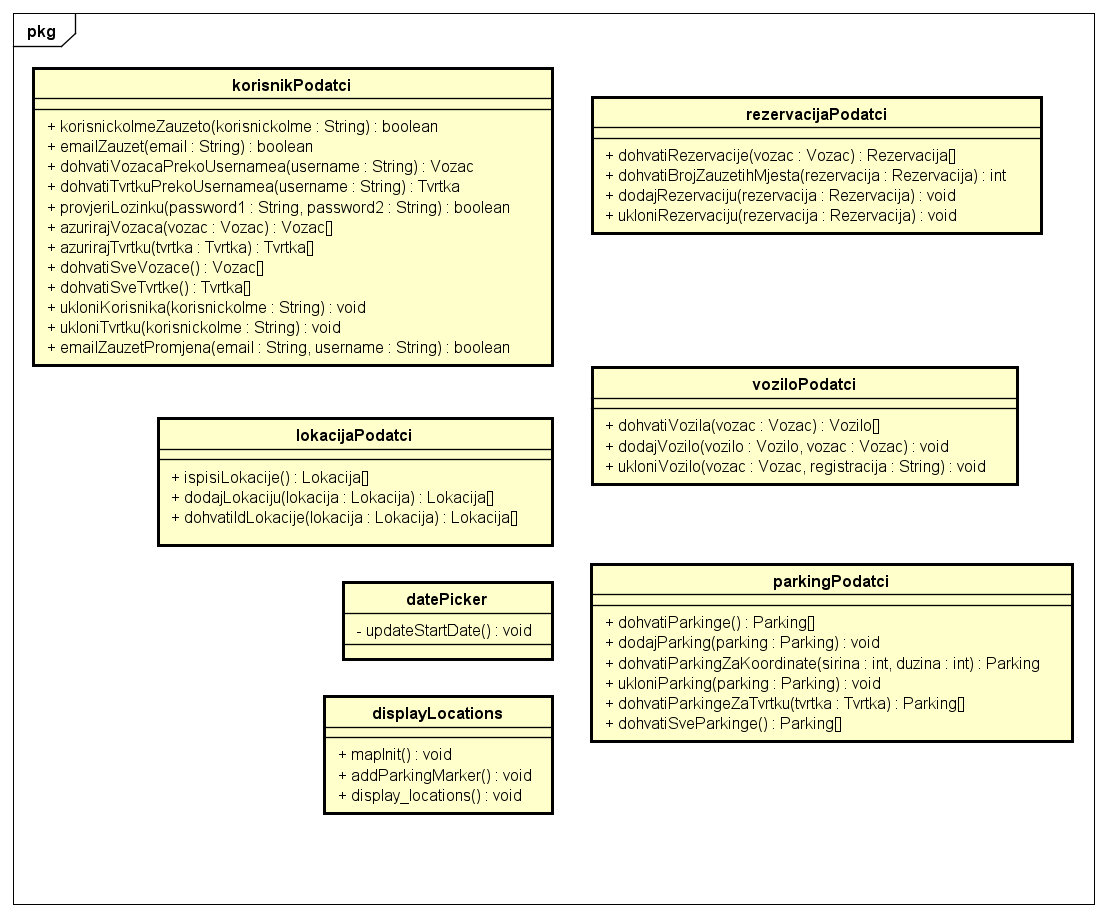
\includegraphics[scale=0.55]{dijagrami/pomocne_funkcije.png} %veličina slike u odnosu na originalnu datoteku i pozicija slike
				\centering
				\caption{Dijagram razreda za pomoćne razrede}
				\label{fig:promjene}
			\end{figure}
		
			\textit{Routeri} su klase koji služe za povezivanje sa \textit{frontendom}, odnosno ostvaruju prikazivanje pug datoteka. Postoje routeri za \textbf{home-page}, stranicu za vozače (\textbf{user.routes}), stranicu za tvrtke (\textbf{company.routes}) te administratora (\textbf{admin.routes}).
			
			\textbf{Napomena:} sve funkcije kao parametre primaju \textit{request} i \textit{response} objekt, te referencu \textit{next} na idući \textit{middleware}\footnote{\textit{middleware} funckije su one funkcije koje imaju pristup \textit{req i res} objektima i idućoj \textit{middleware} funkciji}, no parametri nisu prikazani na dijagramu radi preglednosti.
			
			%unos slike
			\begin{figure}[H]
				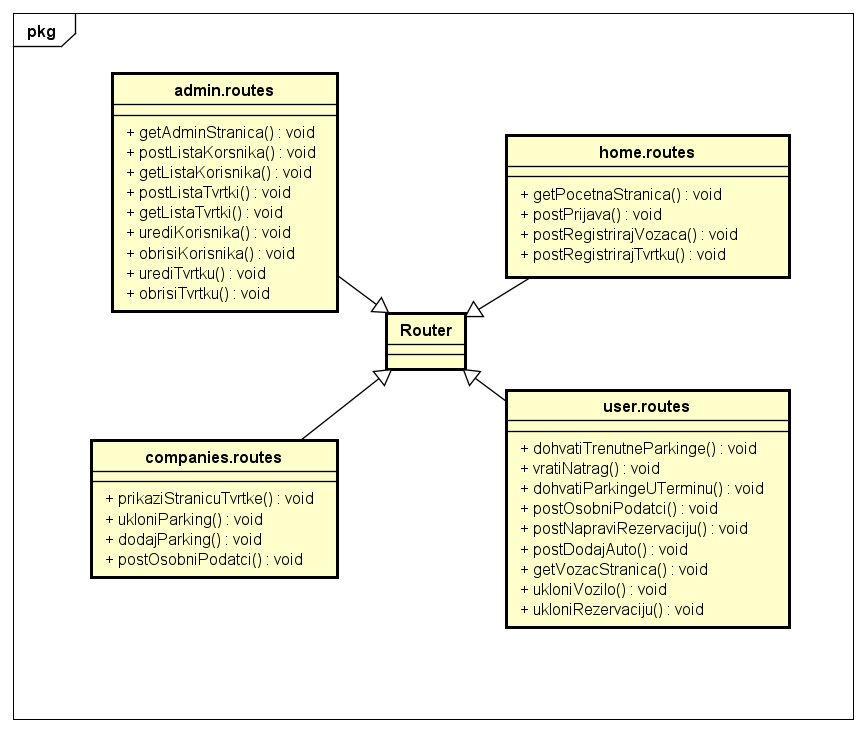
\includegraphics[scale=0.55]{dijagrami/ruteri.png} %veličina slike u odnosu na originalnu datoteku i pozicija slike
				\centering
				\caption{Dijagram razreda za routere}
				\label{fig:promjene}
			\end{figure}
												
			\eject
		
		\section{Dijagram stanja}
			
			Ovaj dijagram stanja prikazuje funkcionalost razreda \textbf{Vozač}. Na web-stranici za vozače (ranije spomenut \textbf{user.routes}) prikazuje se karta pomoću integracije sa \textit{Google Maps APIem}, te više opcija za izabrati koje su naznačene u pravokutnicima. Klik na svaku od njih je otvara, odnosno zatvara te se onda nakon otvaranja prikazuju detalji te opcije. Najkompleksnija opcija je ona za pravljenje rezervacije parking mjesta, jer se u sklopu nje komunicira i sa bazom podataka radi provjere detalja rezervacije i sa poslužiteljem banke gdje se izvršava proces naplate. Greška u bilo kojem dijelu dovršavanja rezervacije otkazuje proces zapisivanja iste u bazu podtaka i njenu naplatu, te usmjerava korisnika nazad na glavnu stranicu gdje može pokušati opet uspješno napraviti rezervaciju.
			
			%unos slike
					\begin{figure}[H]
						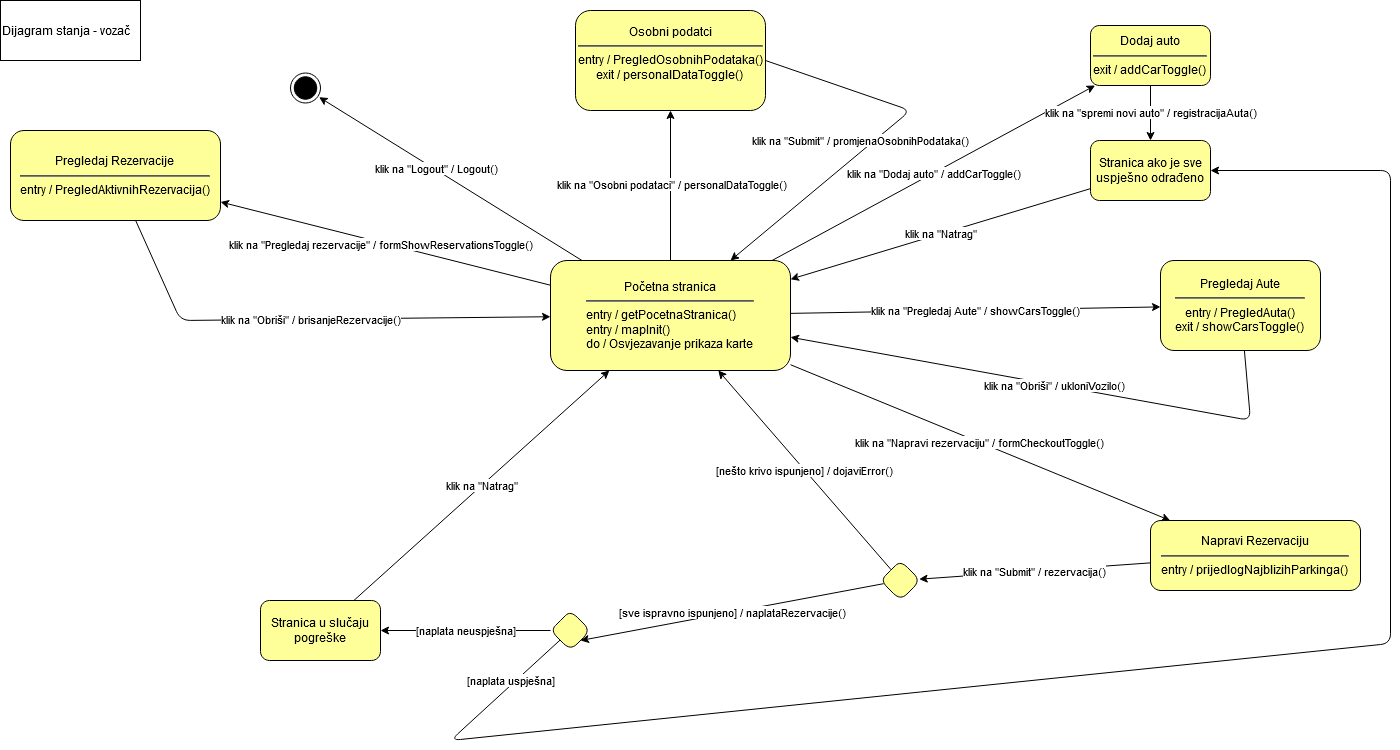
\includegraphics[scale=0.35]{dijagrami/dijagram stanja.png} %veličina slike u odnosu na originalnu datoteku i pozicija slike
						\centering
						\caption{Dijagrama stanja - razred vozač}
						\label{fig:promjene}
					\end{figure}
			
			\eject 
		
		\section{Dijagram aktivnosti}
			 
			 Dio sustava prikazan ovim dijagramom aktivnosti je postupak rezervacije parkinga. Aktivnost započinje (uspješnom) prijavom u sustav. Nakon toga odabire se opcija pravljenja rezervacije gdje se odabire parking i popunjavaju traženi podatci. Važno je napomenuti da se automatski odabire najbliža parking lokacija, koja se onda može ručno izmjeniti po želji korisnika. Nakon ispunjavanja detalja rezervacija se može dovršiti i poslati na naplatu, te ako je sve u redu ona se pamti u bazi podataka i korisnika se obavještava o uspješnoj rezervaciji. Podaci za naplatu se šalju banci na provjeru i izvršavanje naloga pa je neophodno ostvariti sigurnu komunikaciju s tim poslužiteljem radi sigurnosti korisničkih podataka.
			
%unos slike
					\begin{figure}[H]
						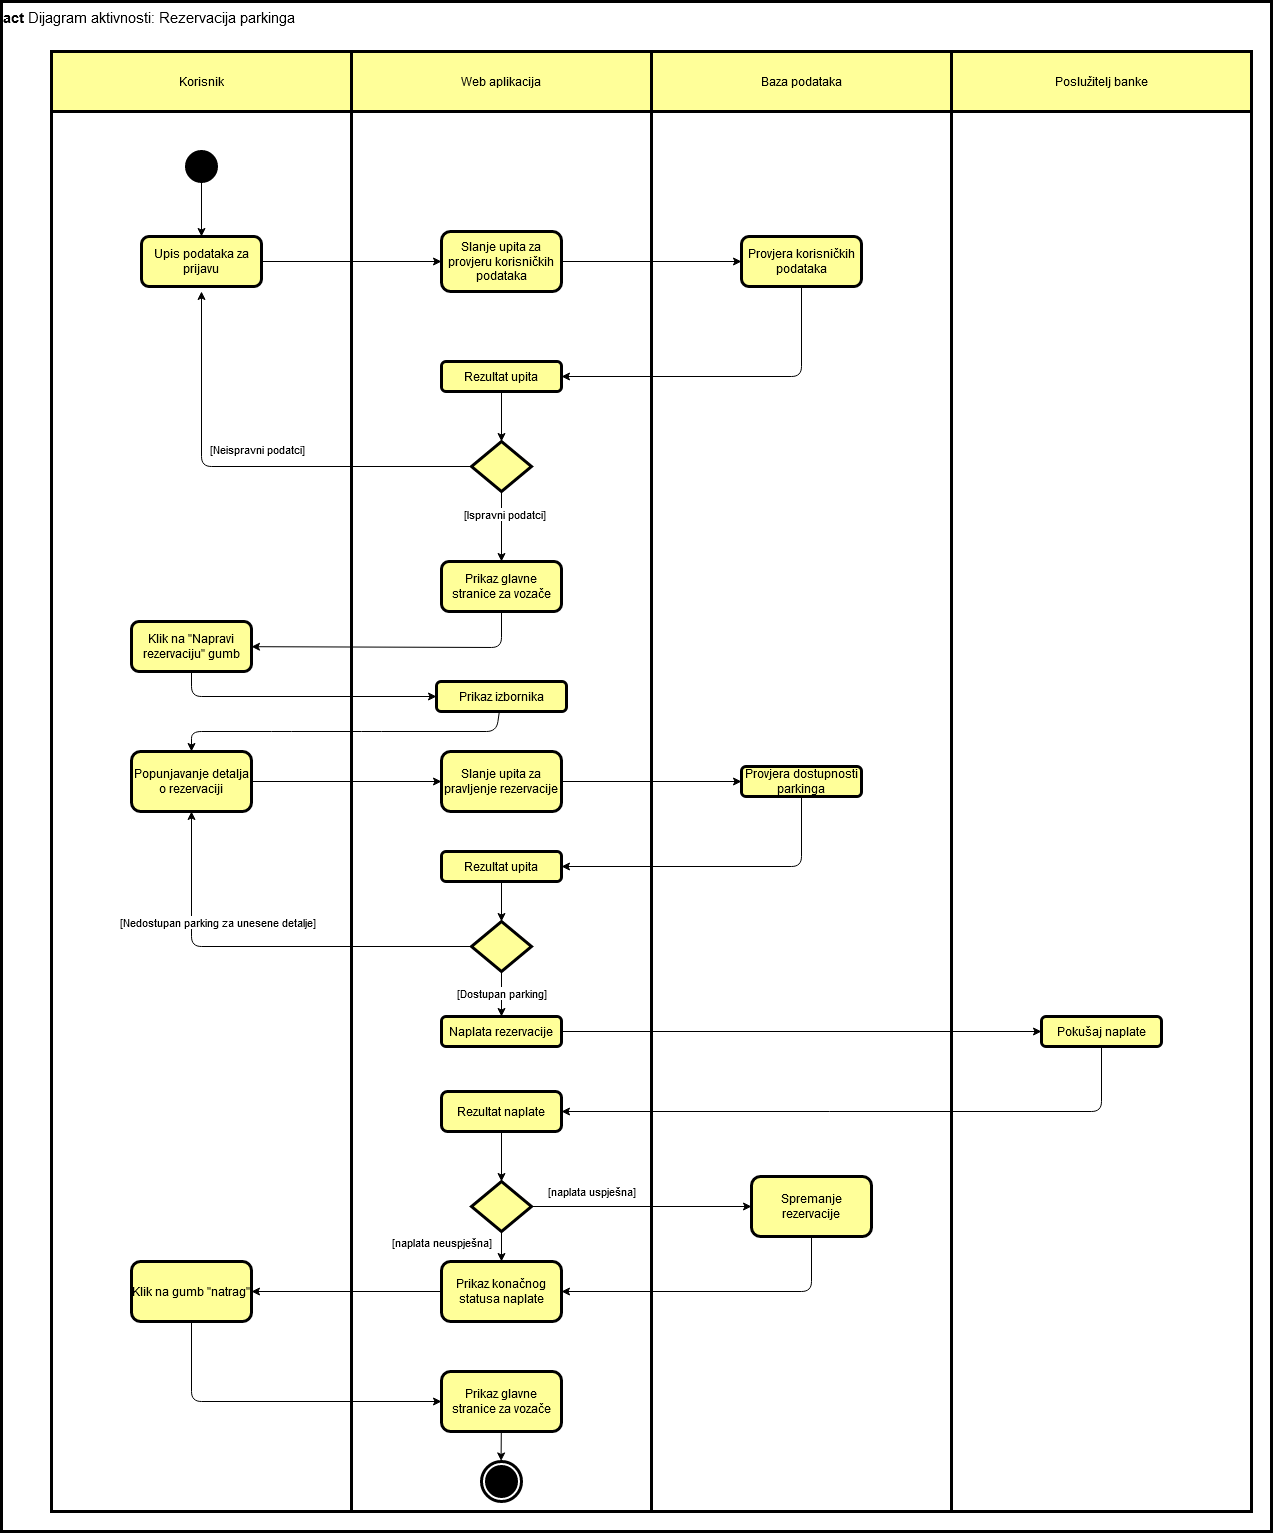
\includegraphics[scale=0.35]{dijagrami/dijagram aktivnosti.png} %veličina slike u odnosu na originalnu datoteku i pozicija slike
						\centering
						\caption{Dijagrama aktivnosti - rezervacija parkinga}
						\label{fig:promjene}
					\end{figure}			
			
			\eject
		\section{Dijagram komponenti}
		
			Na slici je prikazan dijagram komponenti aplikacije. Dijagram prikazuje organizaciju i međuodnos implementacijskih komponenata napravljenih u okviru MVC arhitekture te njihov odnos s okolinom, tj. vanjskim komponentama aplikacije: bazom podataka, \textit{Google Mapsom} i web preglednikom. Web  preglednik komunicira s \textit{routerima} preko REST API  sučelja. Veza između SQL baze podataka i web aplikacije, odnosno njene komponente \textit{podatci} koja dohvađa i obrađuje podatke iz baze podataka, ostvarena je pomoću SQL API sučelja dok je veza s vanjskim servisom \textit{Google Maps} ostavren pomoću GOOGLE MAPS API sučelja.		 
			 
			%unos slike
			 \begin{figure}[H]
				 	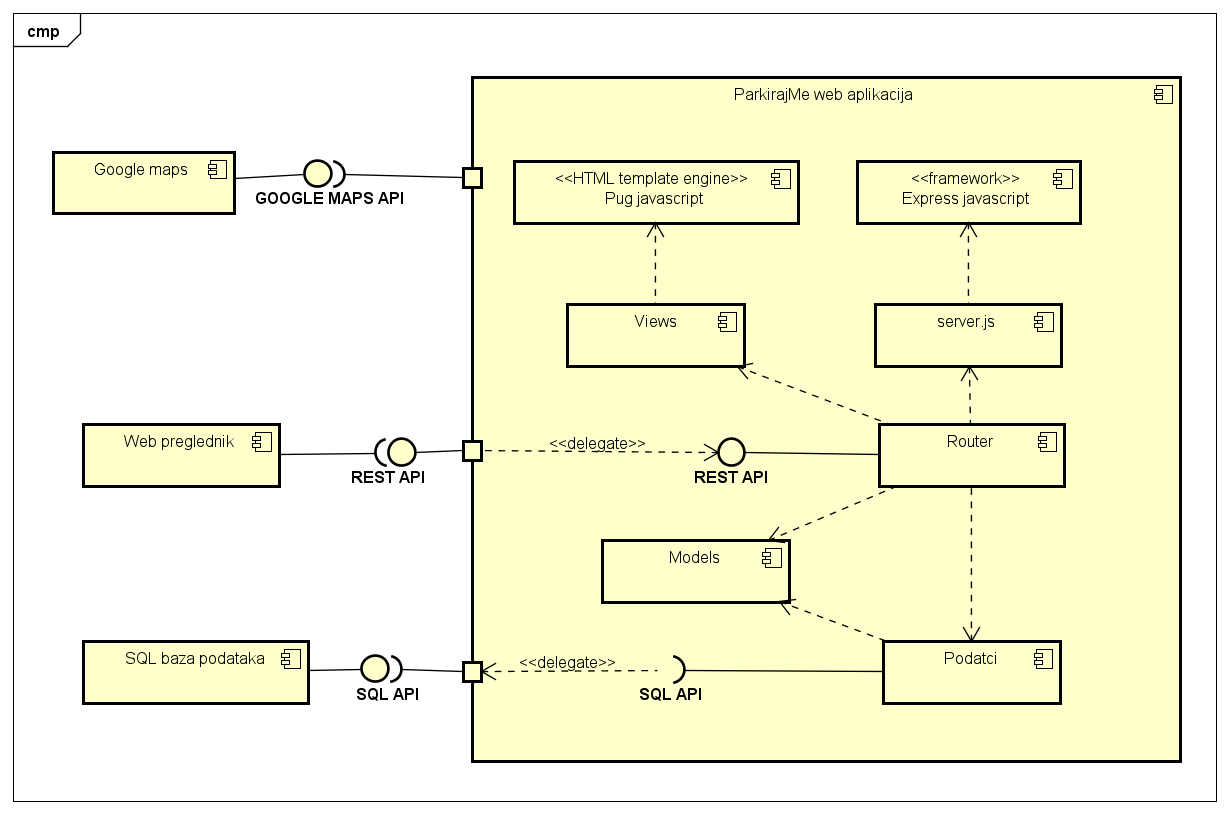
\includegraphics[scale=0.55]{dijagrami/Component Diagram0.png} %veličina slike u odnosu na originalnu datoteku i pozicija slike
				 	\centering
				 	\caption{Dijagram komponenti}
				 	\label{fig:dijagram komponenti}
			 \end{figure}
			 
			 